\documentclass[11pt]{article}

\usepackage{amsmath}
\usepackage{graphicx}
\usepackage{geometry}
\usepackage{float}
\usepackage{tikz}
\usepackage{amsfonts}
\usepackage{enumitem}
\usepackage{caption}
\usepackage{cancel}
\usepackage{subcaption}
\usepackage{booktabs}
\usepackage{multirow}
\usepackage{parskip}

\begin{document}
\section{Data Overview and Initial Exploration}
\begin{itemize}[leftmargin=*]
    \item \textbf{Dataset Source:} Kaggle House Prices: Advanced Regression Techniques
    \item \textbf{Initial Dimensions:} 1460 training samples (rows), 81 feature columns.
    \item \textbf{Data Type Distribution:} Includes 38 numerical features (\texttt{int64}, \texttt{float64}) and 43 categorical/text features (\texttt{object}).
    \item \textbf{Key Observations:} The dataset contains a significant amount of missing values. Furthermore, the large number of initial features makes direct application to linear models prone to overfitting and the curse of dimensionality.
\end{itemize}

\section{Feature Engineering and Missing Value Imputation}
To maximize data value and mitigate noise, we adopted a stratified treatment strategy for missing values rather than blind deletion:

\subsection{Extracting Informative Missingness}
\begin{itemize}[leftmargin=*]
    \item \textbf{Strategy:} Features with extremely high missing rates ($>80\%$, e.g., \texttt{PoolQC}, \texttt{Alley}, \texttt{Fence}, \texttt{MiscFeature}) were transformed into binary features (1: Present / 0: Absent), creating new columns such as \texttt{HasPool}.
    \item \textbf{Decision Rationale:} This approach retains highly valuable signals for house price prediction (e.g., a luxury home possessing a pool) while resolving model instability caused by overly sparse original columns. The original high-missing-rate columns were subsequently dropped.
\end{itemize}

\subsection{Numerical Feature Imputation}
\begin{itemize}[leftmargin=*]
    \item \textbf{Strategy:} Implemented an automated imputation mechanism based on \textbf{Skewness}. The absolute skewness of each numerical feature was evaluated:
    \begin{itemize}
        \item \textbf{Highly Skewed ($|\text{Skewness}| > 1.0$):} Indicates the presence of extreme outliers (e.g., ultra-luxury mansions). Imputed using the \textbf{median}.
        \item \textbf{Roughly Symmetric ($|\text{Skewness}| \leq 1.0$):} Imputed using the \textbf{mean}.
    \end{itemize}
    \item \textbf{Decision Rationale:} This dynamic strategy adapts to the underlying distribution of each individual feature, preserving the original statistical properties much more accurately than a uniform median imputation.
\end{itemize}

\subsection{Categorical Feature Imputation}
\begin{itemize}[leftmargin=*]
    \item \textbf{Strategy:} Abandoned uniform mode imputation in favor of a dual-track decision mechanism combining \textbf{statistical distribution} and \textbf{domain knowledge}:
    \begin{itemize}
        \item \textbf{Extremely Low Missing Rate with Dominant Class (e.g., \texttt{Electrical}):} With a missing rate of only 0.1\% and a mode dominance of 91.4\%, this indicates random human omission. Imputed using the \textbf{mode}.
        \item \textbf{Domain-Specific Correlated Missingness (e.g., \texttt{Garage} and \texttt{Bsmt} families):} Observed uniform missing rates across related features (5.5\% for garage, 2.5\% for basement). Domain knowledge dictates this represents the physical absence of the facility (i.e., "No Garage"), not missing data. Forced mode imputation would artificially synthesize non-existent amenities, thus these were imputed with \textbf{"None"}.
        \item \textbf{High Missing Rate Features (e.g., \texttt{MasVnrType}, \texttt{FireplaceQu}):} Missing rates between 40\%-60\% indicate the general absence of these specific upgrades. Imputed with \textbf{"None"}.
    \end{itemize}
    \item \textbf{Decision Rationale:} This prevents distribution distortion caused by blind mode imputation and ensures the engineered features strictly adhere to real-world real estate logic, thereby increasing the reliability of the predictive model.
\end{itemize}

\section{Categorical Encoding}
Since machine learning algorithms (Linear, Ridge, Lasso, SVR) cannot directly process text, strings must be converted into numerical representations:
\begin{itemize}[leftmargin=*]
    \item \textbf{Strategy:} Applied \textbf{One-Hot Encoding} utilizing \texttt{pd.get\_dummies(drop\_first=True)}.
    \item \textbf{Dimensionality Change:} After expanding over 40 categorical features, the total number of features expanded from 77 to 241.
    \item \textbf{Decision Rationale:} Using \texttt{drop\_first=True} drops the first category level to bypass the \textbf{Dummy Variable Trap}. This ensures the stability of subsequent linear regression models and mitigates multicollinearity issues.
\end{itemize}

\section{Target Variable and Feature Splitting}
\begin{itemize}[leftmargin=*]
    \item \textbf{Feature Matrix (X) and Target Variable (y):} \texttt{SalePrice} was isolated as \texttt{y}, while the remaining 240 features constituted the feature matrix \texttt{X}.
    \item \textbf{Train/Test Split:} Utilized \texttt{scikit-learn} to split the dataset at an 80:20 ratio (Train: 80\%, Test: 20\%). A fixed \texttt{random\_state} was configured to guarantee consistency and reproducibility in future model comparison benchmarks.
\end{itemize}

\subsection{Baseline Linear Regression}
% 在此撰寫 Baseline 訓練過程與 RMSE 表現
\subsection{Baseline Linear Regression (OLS)}

To establish a rigorous performance benchmark for evaluating subsequent regularized models and advanced ensemble algorithms, this study first implemented a baseline model utilizing \textbf{Ordinary Least Squares (OLS)} linear regression.

\subsubsection{Target Variable Transformation}
Initial exploratory data analysis revealed that the target variable, \texttt{SalePrice}, exhibited a significant right-skewed distribution, as illustrated in the left panel of \textbf{Figure \ref{fig:price_transform}}. Such skewness can lead linear models to be overly sensitive to high-value outliers, potentially compromising generalizability.

To address this, a log-transformation was applied: $y = \log(1 + \text{SalePrice})$. As shown in the right panel of \textbf{Figure \ref{fig:price_transform}}, the transformed data approximates a normal distribution (Gaussian-like). This transformation satisfies the homoscedasticity and normality assumptions of linear regression and converts absolute price errors into relative percentage errors, ensuring more robust weight estimation across different price tiers.

\begin{figure}[H]
    \centering
    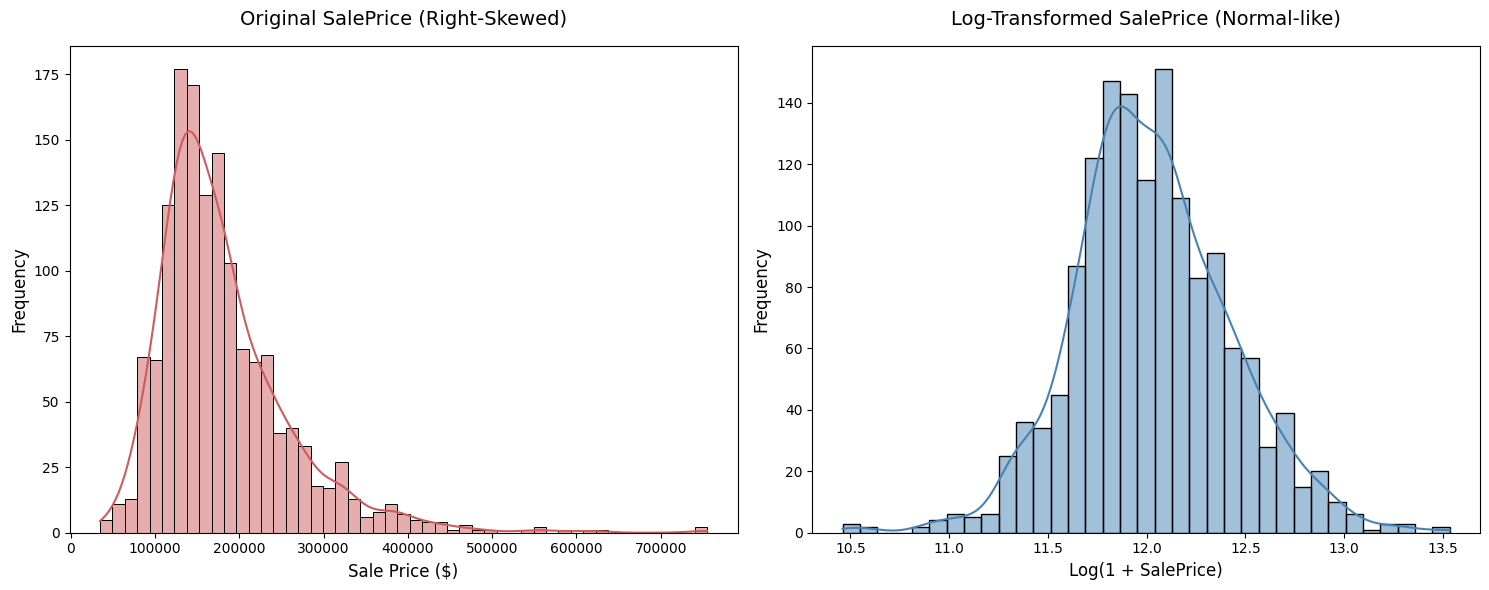
\includegraphics[width=0.85\textwidth]{../picture/price_transform.png}
    \caption{Distribution of SalePrice: Original skewed data (left) vs. Log-transformed normal-like data (right).}
    \label{fig:price_transform}
\end{figure}

\subsubsection{Model Evaluation and Visual Analysis}
The baseline model was evaluated using \textbf{5-Fold Cross-Validation} on the development set (80\% of the data) with a shuffle mechanism (\texttt{random\_state=42}) to ensure stability.

\vspace{0.5em}
\noindent \textbf{Baseline Model Diagnostics:}\\
To comprehensively evaluate the performance of the Baseline OLS model, we analyzed its predictive distribution and stability through two complementary visualizations, as shown in Figure \ref{fig:baseline_diagnostics}.

\begin{figure}[H]
     \centering
     \begin{subfigure}[b]{0.48\textwidth}
         \centering
         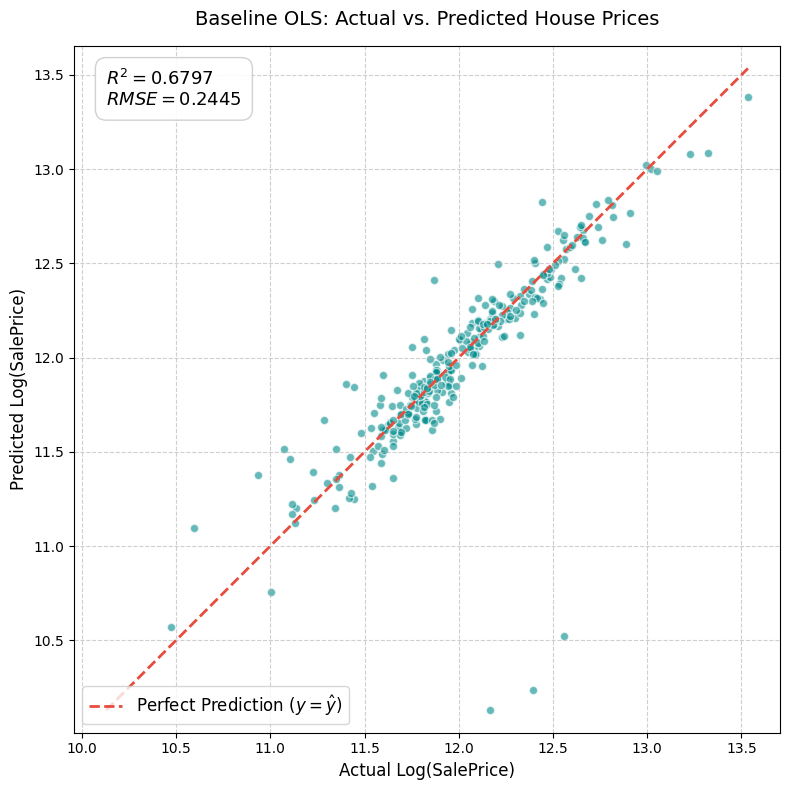
\includegraphics[width=\textwidth]{../picture/baseline_predict_actual.png}
         \caption{Actual vs. Predicted Plot}
         \label{fig:pred_actual}
     \end{subfigure}
     \hfill
     \begin{subfigure}[b]{0.48\textwidth}
         \centering
         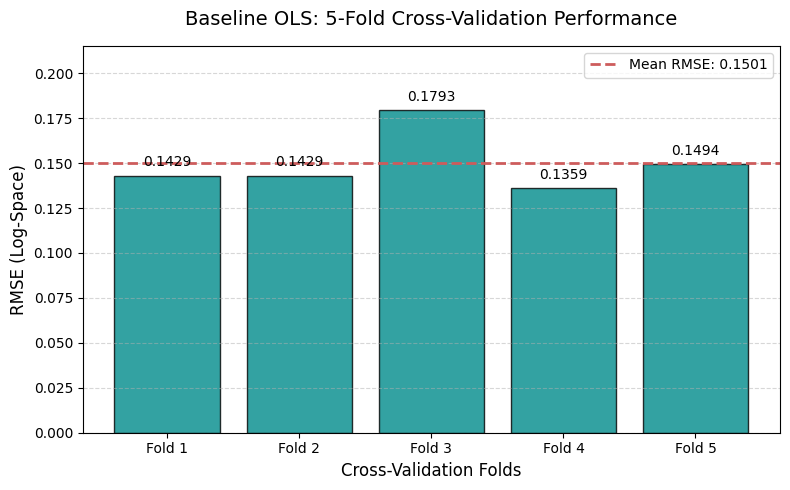
\includegraphics[width=\textwidth]{../picture/Basline_cross_validation.png}
         \caption{5-Fold Cross-Validation Scores}
         \label{fig:cv_scores}
     \end{subfigure}
     \caption{Diagnostic visualizations of the Baseline OLS model, illustrating high variance and weight instability.}
     \label{fig:baseline_diagnostics}
\end{figure}

\noindent Based on the combined evidence from Figure \ref{fig:baseline_diagnostics}, we identify the following challenges:

\begin{itemize}[leftmargin=*]
    \item \textbf{Catastrophic Underprediction and Weight Instability:} As illustrated in Figure 2a, the unregularized OLS model demonstrates severely inadequate predictive performance, yielding a sub-optimal $R^2$ score of only 0.6797. Beyond the general dispersion of predictions, the model suffers from extreme localized failures. Specifically, a cluster of three standard properties with actual log values around 12.5 were severely underpredicted, plummeting to a range between $\sim$10.5 and $\sim$9.5. This magnitude of error across multiple data points proves that the OLS model systemically overreacts to specific feature combinations in the high-dimensional space, leading to erratic coefficient estimates and overall model collapse.
    \item \textbf{Performance Fluctuation in CV:} Figure \ref{fig:cv_scores} confirms this instability, with RMSE scores fluctuating violently between Fold 3 (0.1793) and Fold 4 (0.1359). This sensitivity to data splits is a hallmark of \textbf{High Variance} and \textbf{Overfitting}.

\begin{figure}[H]
    \centering
    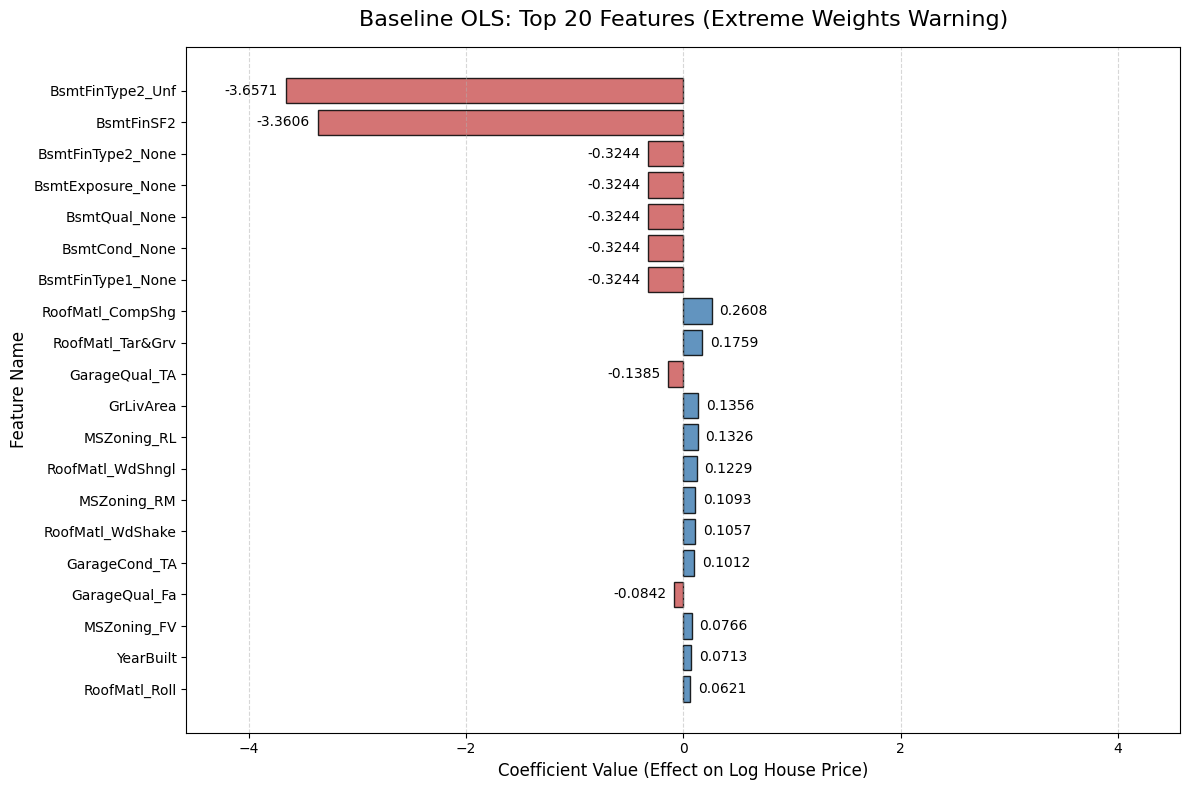
\includegraphics[width=0.8\textwidth]{../picture/baseline_influential_features.png}
    \caption{Top 20 Influential Features of the Baseline OLS Model}
    \label{fig:baseline_features}
\end{figure}

 \item \textbf{The Root Cause --- Multicollinearity and Predictive Landmines:} To diagnose the root cause of this model collapse, we analyzed the coefficient weights of the Baseline OLS model (Figure \ref{fig:baseline_features}). The distribution reveals a severe case of algorithmic hijacking by sparse and highly collinear categorical variables. Instead of relying on fundamental structural metrics (e.g., \texttt{GrLivArea} is marginalized with a mere weight of 0.1356), the unregularized model inflates the coefficients of specific basement features to absurd magnitudes.

Most notably, the model creates catastrophic ``predictive landmines'' by assigning extremely aggressive negative weights to features like \texttt{BsmtFinType2\_Unf} (-3.6571) and \texttt{BsmtFinSF2} (-3.3606). Furthermore, the model explicitly suffers from \textit{Perfect Multicollinearity}, as evidenced by a block of five basement-related \texttt{\_None} features (e.g., \texttt{BsmtQual\_None}) receiving identical weights of -0.3244. Because OLS lacks a regularization penalty to handle correlated features securely, it arbitrarily distributes weights across these identical indicator variables.

This over-fitting mechanism directly explains the catastrophic underprediction observed in Figure 2a. The three severely underpredicted properties in the validation set likely possessed a specific basement configuration that triggered these unconstrained negative coefficients. These massive penalties violently dragged their predicted log-prices down to $\sim$9.75, completely overriding the properties' true structural value and causing the overall variance to spike.

\end{itemize}

\begin{table}[H]
\centering
\label{tab:baseline_results}
\begin{tabular}{lc}
\hline
\textbf{Metric} & \textbf{RMSE (Log-Space)} \\ \hline
5-Fold CV Average RMSE & 0.1501 \\
Final Test RMSE & 0.2445 \\ \hline
\end{tabular}
\caption{Performance Summary of Baseline Linear Regression}
\end{table}

As summarized in Table 1, although the Baseline OLS model achieves a seemingly reasonable mean RMSE of 0.1501 during 5-fold cross-validation, its performance severely degrades when evaluated on the unseen test dataset, with the RMSE spiking drastically to 0.2445. Notably, this test error far exceeds even the worst-performing fold from the cross-validation phase (0.1793). This glaring discrepancy between validation and test generalization is a clear indicator of severe overfitting. Consequently, these findings establish a definitive necessity for implementing \textbf{Ridge and Lasso Regression} to constrain the coefficient magnitudes and restore overall model robustness.

\subsection{L1 and L2 Regularization (Lasso and Ridge)}
% 在此撰寫 Ridge 與 Lasso 的特性、Alpha 參數挑選，以及 L1 帶來的特徵稀疏性
\subsection{Hyperparameter Tuning: Alpha Path Analysis}
To determine the optimal regularization strength, we performed a log-scale grid search using 5-Fold Cross-Validation for both Lasso and Ridge models.

\begin{figure}[H]
     \centering
     \begin{subfigure}[b]{0.48\textwidth}
         \centering
         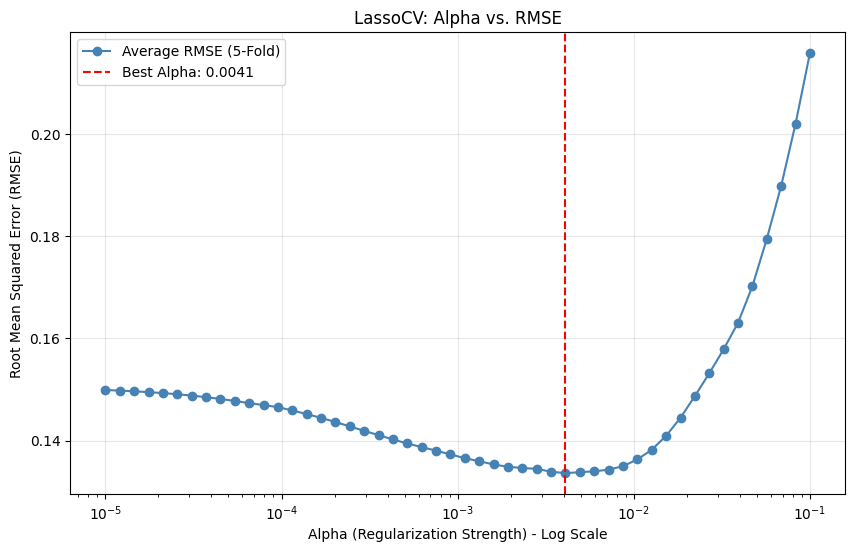
\includegraphics[width=\textwidth]{../picture/Lasso_alpha.png}
         \caption{LassoCV: Optimal $\alpha = 0.0041$}
         \label{fig:lasso_alpha}
     \end{subfigure}
     \hfill
     \begin{subfigure}[b]{0.48\textwidth}
         \centering
         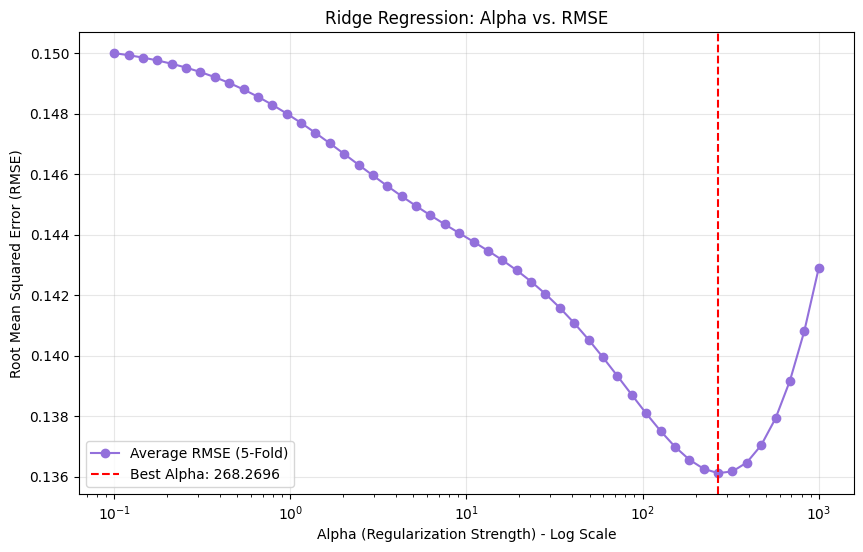
\includegraphics[width=\textwidth]{../picture/Ridge_alpha.png}
         \caption{RidgeCV: Optimal $\alpha \approx 268.2696$}
         \label{fig:ridge_alpha}
     \end{subfigure}
     \caption{Hyperparameter tuning paths. The red dashed lines indicate the $\alpha$ values that minimize the mean Cross-Validation RMSE.}
     \label{fig:alpha_tuning}
\end{figure}

\begin{itemize}[leftmargin=*]
    \item \textbf{Under-regularization (Left side):} At extremely low $\alpha$ values, the penalty is negligible, and the models behave similarly to the unconstrained Baseline OLS. They suffer from high variance by capturing too much dataset noise, leading to elevated cross-validation errors.
    \item \textbf{Over-regularization (Right side):} Conversely, as $\alpha$ increases excessively, the models face severe penalties. Critical feature weights are shrunk to zero (Lasso) or near-zero (Ridge), resulting in high bias and underfitting, which causes the RMSE to spike drastically.
    \item \textbf{The Optimal Sweet Spot (Red dashed line):} The global minimum on each curve represents the optimal balance between bias and variance. Notably, Lasso achieves its optimum at a highly sensitive, small scale ($\alpha = 0.0041$), whereas Ridge optimizes at a vastly larger scale ($\alpha \approx 268.2696$). This discrepancy is driven by their mathematical formulations: the L1 norm (absolute sum) in Lasso applies a much harsher shrinkage per unit of $\alpha$ compared to the L2 norm (squared sum) in Ridge.
\end{itemize}

\noindent By systematically selecting these specific $\alpha$ parameters, we ensure the models effectively filter out idiosyncratic noise while retaining robust predictive signals.

\subsection{Model Stabilization: Cross-Validation Performance}

\begin{figure}[H]
     \centering
     \begin{subfigure}[b]{0.48\textwidth}
         \centering
         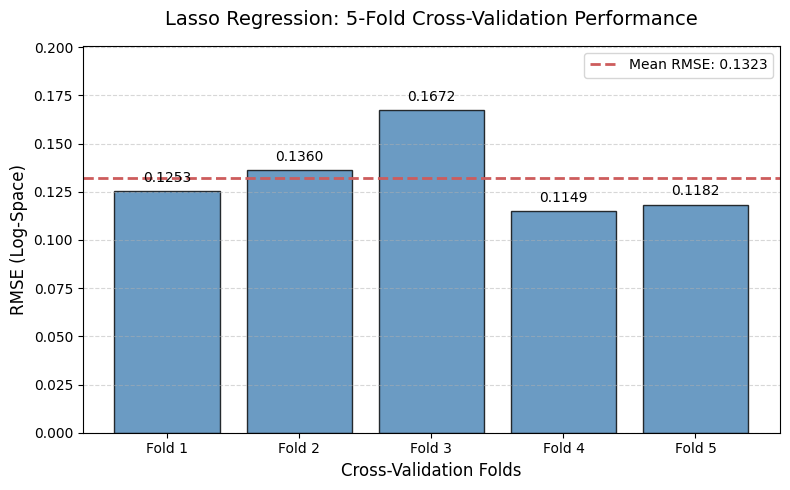
\includegraphics[width=\textwidth]{../picture/Lasso_cross_validation.png}
         \caption{Lasso CV (Mean RMSE: 0.1323)}
         \label{fig:lasso_cv}
     \end{subfigure}
     \hfill
     \begin{subfigure}[b]{0.48\textwidth}
         \centering
         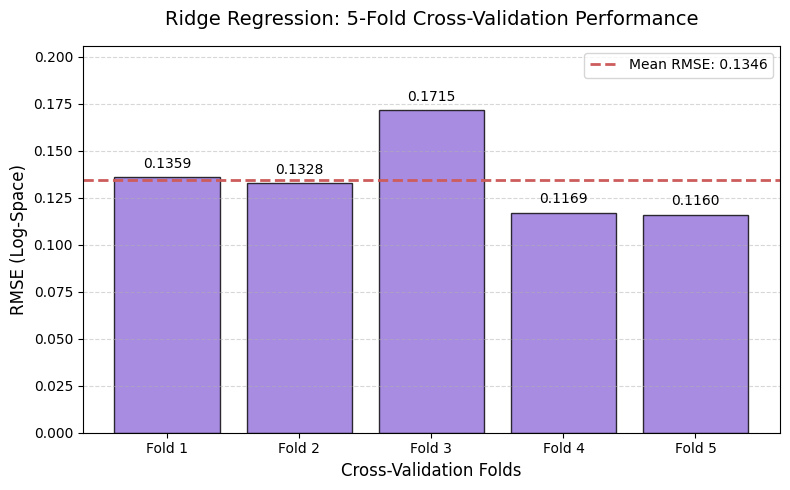
\includegraphics[width=\textwidth]{../picture/Ridge_cross_validation.png}
         \caption{Ridge CV (Mean RMSE: 0.1346)}
         \label{fig:ridge_cv}
     \end{subfigure}
     \caption{Cross-Validation performance of regularized models.}
     \label{fig:regularized_cv}
\end{figure}

\begin{itemize}[leftmargin=*]
\item As shown in \textbf{Figure 4}, both models achieved lower overall mean RMSEs (Lasso: 0.1323, Ridge: 0.1346) compared to the unregularized baseline, successfully dampening the extreme predictive fluctuations across most data splits. 
\item However, a critical observation must be made regarding the persistent instability in \textbf{Fold 3}. Despite the application of optimal L1 and L2 penalty terms, Fold 3 exhibits a disproportionately high error (Lasso: 0.1672, Ridge: 0.1715) relative to the other folds. 
\item This prominent residual variance reveals a fundamental limitation: while regularization effectively constrains coefficient magnitudes to prevent overfitting, it cannot fully mitigate variance if the underlying data slice contains severe outliers or structural anomalies. The resilient spike in Fold 3 suggests the presence of complex, non-linear relationships within that specific validation subset that fundamentally violate the assumptions of linear models, warranting future exploration with robust, non-linear algorithms (e.g., Tree-based models).
\end{itemize}

\subsection{Outlier Mitigation in Individual Predictions}

While the cross-validation metrics reveal the macro-level behavior of the regularized models across different data splits, analyzing the Actual vs. Predicted scatter plots provides crucial micro-level insights into individual property valuations. 

\vspace{0.5em}
\noindent This visual diagnostic reveals the true triumph of regularization: the elimination of catastrophic weight instability.

\begin{figure}[H]
     \centering
     \begin{subfigure}[b]{0.48\textwidth}
         \centering
         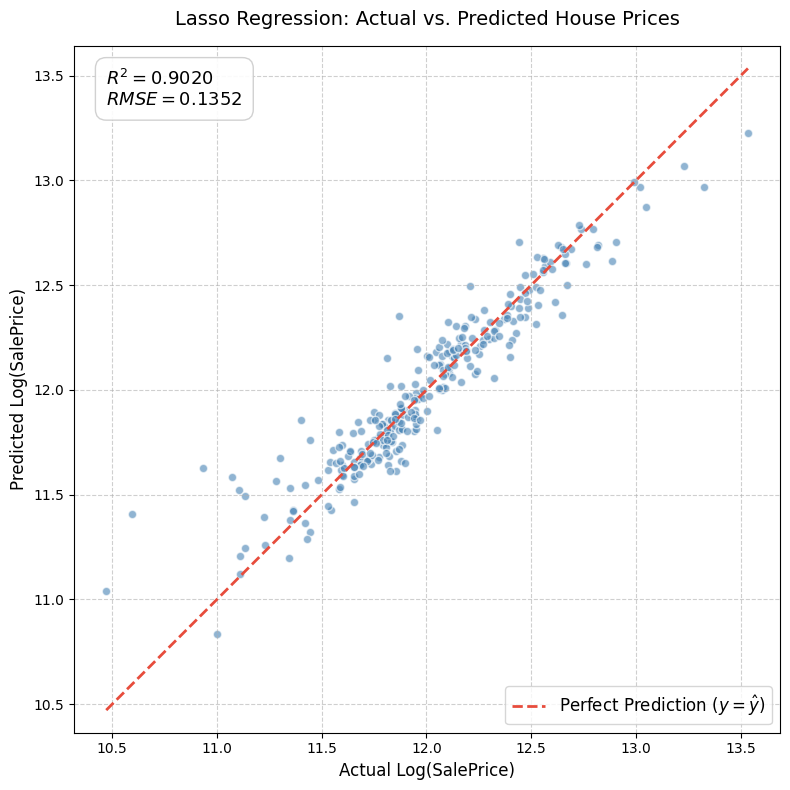
\includegraphics[width=\textwidth]{../picture/lasso_predict_actual.png}
         \caption{Lasso Regression}
         \label{fig:lasso_pred}
     \end{subfigure}
     \hfill
     \begin{subfigure}[b]{0.48\textwidth}
         \centering
         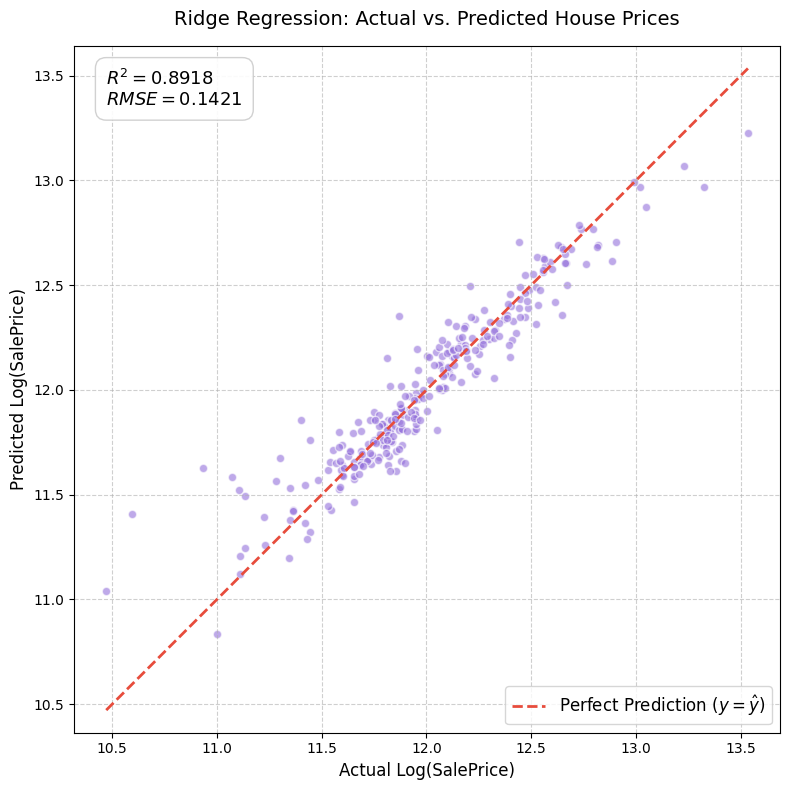
\includegraphics[width=\textwidth]{../picture/ridge_predict_actual.png}
         \caption{Ridge Regression}
         \label{fig:ridge_pred}
     \end{subfigure}
     \caption{Actual vs. Predicted distributions for regularized models. Both techniques successfully eliminate the severe underprediction outliers observed in the baseline OLS.}
     \label{fig:regularized_scatter}
\end{figure}

As illustrated in Figure \ref{fig:regularized_scatter}, both Lasso and Ridge models successfully bounded the predictions closely to the 45-degree reference line, marking a dramatic quantitative and qualitative recovery from the Baseline OLS. Most notably, the catastrophic underprediction observed in the baseline—where a cluster of three standard properties with actual log values around 12.5 were severely underestimated to a range between $\sim$10.5 and $\sim$9.5—has been completely eradicated. 

This visual stabilization is the direct result of L1 and L2 regularizations deactivating the ``predictive landmines'' caused by sparse categorical features. The effectiveness of this safety net is reflected in a significant leap in overall predictive power: the aggregate $R^2$ score surged from a sub-optimal 0.6797 in the Baseline OLS to an impressive 0.9020 for Lasso and 0.8918 for Ridge. 

Even if these regularization techniques could not perfectly flatten the variance across all data folds (as noted in Section 4.5), they effectively prevented the model from overreacting to idiosyncratic noise and multicollinearity. By constraining the coefficient magnitudes, we ensured that no individual property suffers from the extreme, erratic valuation errors that characterized the unregularized OLS model.

\subsection{Feature Insights: Sparsity vs. Shrinkage}
While both models improved predictive stability, their handling of the 240-dimensional feature space differed fundamentally due to their distinct penalty terms.

\begin{figure}[H]
     \centering
     \begin{subfigure}[b]{0.48\textwidth}
         \centering
         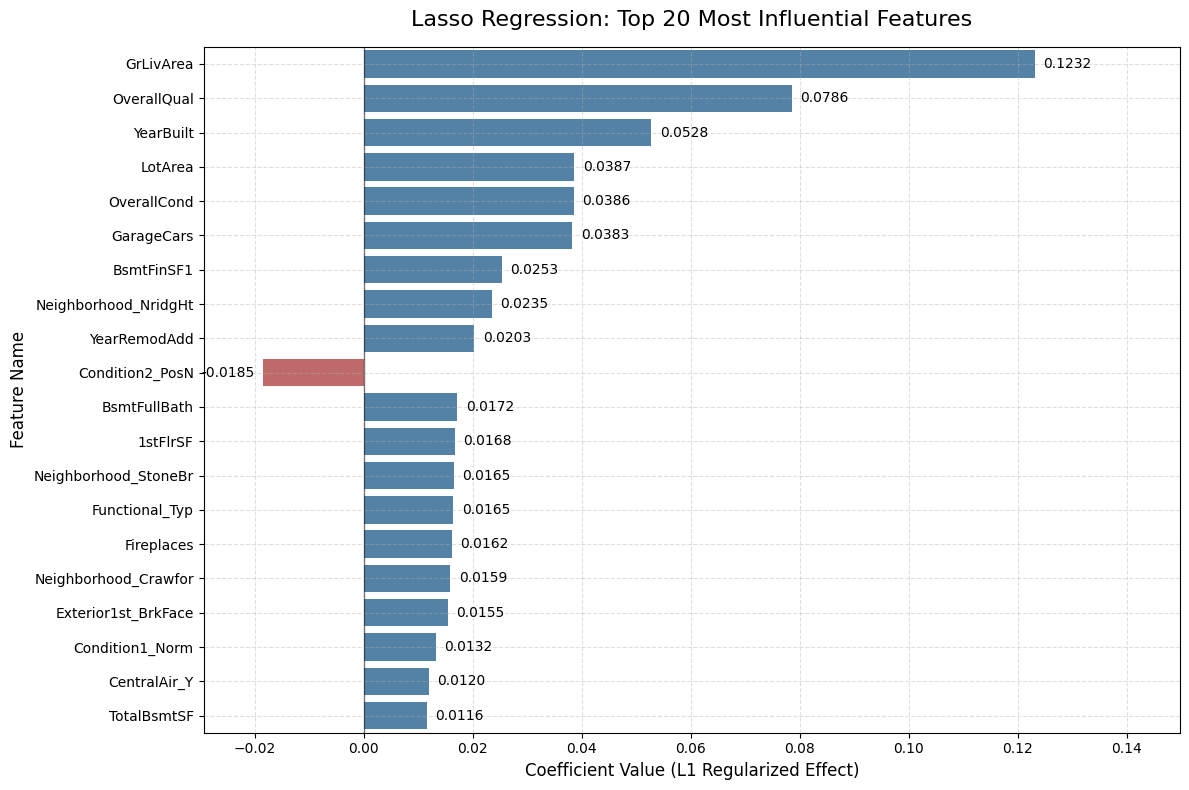
\includegraphics[width=\textwidth]{../picture/lasso_influential_features.png}
         \caption{Lasso: Feature Selection (Sparsity)}
         \label{fig:lasso_features}
     \end{subfigure}
     \hfill
     \begin{subfigure}[b]{0.48\textwidth}
         \centering
         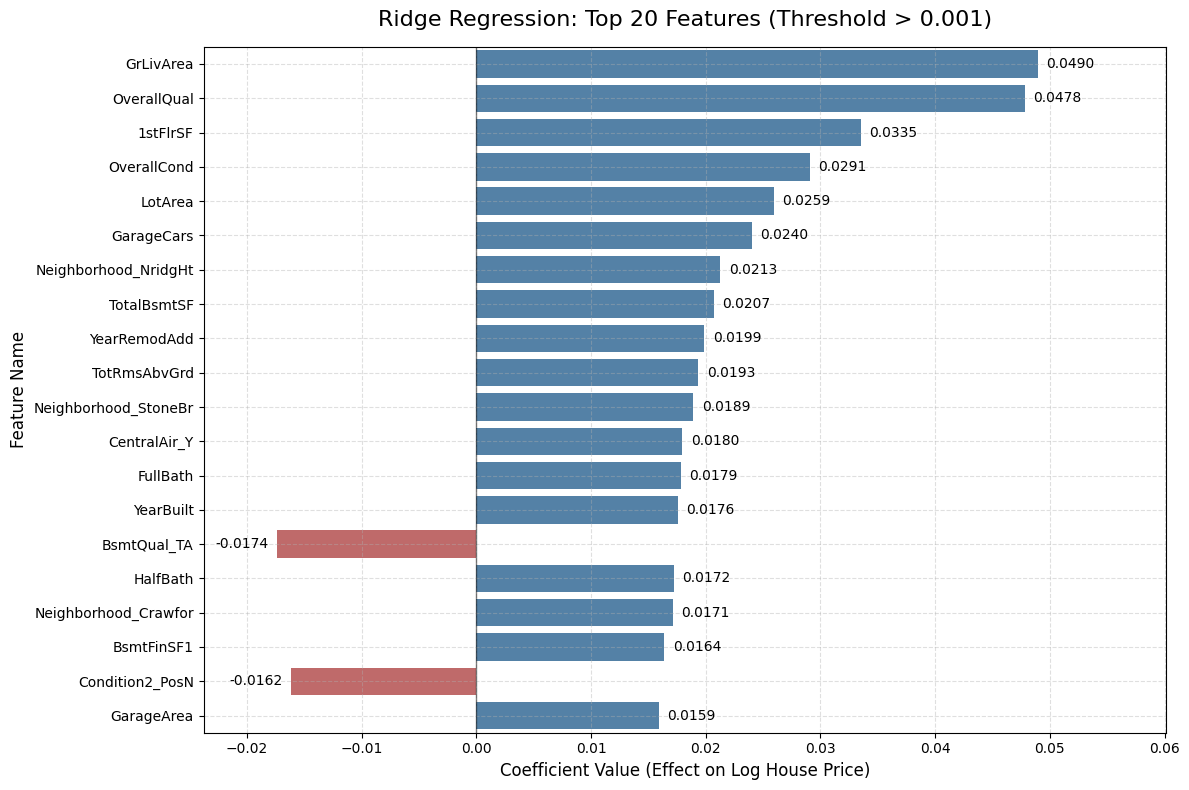
\includegraphics[width=\textwidth]{../picture/Ridge_influential_features.png}
         \caption{Ridge: Coefficient Shrinkage}
         \label{fig:ridge_features}
     \end{subfigure}
     \caption{Top 20 most influential features.}
     \label{fig:feature_importance}
\end{figure}

\begin{table}[H]
    \centering
    \renewcommand{\arraystretch}{1.2}
    \begin{tabular}{l c c c c l}
        \toprule
        \textbf{Model} & \textbf{Penalty} & \textbf{Total Features} & \textbf{Retained} & \textbf{Suppressed} & \textbf{Criteria} \\
        \midrule
        Lasso & L1 & 250 & \textbf{92} & 158 & Coef $= 0$ \\
        Ridge & L2 & 250 & \textbf{212} & 38 & $\mid$Coef$\mid < 0.001$ \\
        \bottomrule
    \end{tabular}
    \caption{Quantitative comparison of feature selection and shrinkage effects between Lasso and Ridge regression.}
    \label{tab:feature_selection}
\end{table}

\subsubsection{Quantitative Impact: Sparsity vs. Shrinkage}
As quantified in \textbf{Table 2}, the fundamental difference between L1 and L2 regularization is explicitly revealed in their final active feature counts. Lasso effectively acts as a strict automated feature selector; it aggressively forces the coefficients of 158 less informative or highly collinear features to exactly zero, retaining a sparse subset of only 92 critical predictors. In contrast, Ridge employs continuous coefficient shrinkage. By retaining 212 features with absolute weights greater than 0.001, Ridge demonstrates its mathematical preference to distribute the penalty evenly across correlated variables rather than eliminating them entirely.

\subsubsection{Qualitative Consensus on Market Drivers}
Despite their opposing mathematical mechanics, Figure \ref{fig:feature_importance} demonstrates that both regularized models reach a striking consensus on the most impactful drivers of property value. By eliminating these sparse coefficient anomalies, regularization restores focus to fundamental real estate metrics.

\begin{itemize}
    \item \textbf{Consensus on Primary Additions (Structural Dominance):} Unlike the unregularized baseline, both Lasso and Ridge correctly identify core structural metrics as the absolute primary drivers of house prices. Above-ground living area (\texttt{GrLivArea}) and overall material/finish quality (\texttt{OverallQual}) decisively dominate the top two positions across both algorithms.
    
    \item \textbf{Consensus on Detractions:} Both models agree on specific adverse conditions that penalize property value. Notably, \texttt{Condition2\_PosN} (proximity to specific off-site features) is consistently identified as a primary value detractor in both Lasso and Ridge architectures.
    
    \item \textbf{Algorithmic Behavior: Aggressive Selection vs. Symmetric Shrinkage:} The charts brilliantly visualize the theoretical difference between L1 and L2 penalties. Lasso (L1) aggressively concentrates predictive power into a single primary feature, assigning \texttt{GrLivArea} a dominant weight of 0.1232. In contrast, Ridge (L2) enforces a much stricter overall coefficient shrinkage (max weight only 0.0490) and distributes the predictive importance more symmetrically across correlated features, giving substantial weights to both \texttt{GrLivArea} (0.0490) and \texttt{1stFlrSF} (0.0335).
\end{itemize}

Ultimately, this dual analysis highlights the strategic trade-off in regularization: Lasso provides a highly interpretable, streamlined model by isolating the absolute strongest signals and enforcing sparsity, whereas Ridge preserves the nuanced, collective predictive power of the entire feature space while safely dampening its overall variance.
\subsubsection{Overall Performance: Regularized Models vs. Baseline}

To conclusively evaluate the effectiveness of the regularized models, we compared their cross-validation stability, final predictive accuracy on the test set, and real-world business interpretability. 

\vspace{0.5em}
\noindent Since our models were trained on a log-transformed target variable ($y = \log(1 + \text{SalePrice})$), the resulting Log-RMSE inherently approximates the relative error. To translate this statistical variance into an intuitive business metric, we explicitly converted the Log-RMSE into a \textbf{Mean Percentage Error} using the following exponential transformation:

\begin{equation}
    \text{Mean Percentage Error} = \left( e^{\text{RMSE}_{\text{log}}} - 1 \right) \times 100\%
\end{equation}

\noindent This formula mathematically maps the variance observed in the logarithmic space directly to the expected percentage deviation in real-world dollar valuations.

\begin{table}[H]
    \centering
    \renewcommand{\arraystretch}{1.2}
    \begin{tabular}{lccc}
        \toprule
        \textbf{Model} & \textbf{CV RMSE (Log)} & \textbf{Test RMSE (Log)} & \textbf{MPE} \\
        \midrule
        Baseline OLS & 0.1501 & 0.2445 & 27.69\% \\
        Lasso (L1)   & \textbf{0.1323} & \textbf{0.1352} & \textbf{14.48\%} \\
        Ridge (L2)   & 0.1346 & 0.1421 & 15.27\% \\
        \bottomrule
    \end{tabular}
    \caption{Performance comparison across linear models.}
    \label{tab:model_comparison}
\end{table}

\noindent As summarized in \textbf{Table \ref{tab:model_comparison}}, the application of regularization significantly stabilized the training process and improved generalization. 

\vspace{0.5em}
\noindent More importantly, evaluating the models using Mean Percentage Error reveals the tangible real-world impact of our feature engineering and hyperparameter tuning. The Baseline OLS model suffers from an unacceptable average error margin of 27.69\%, rendering it unsuitable for practical real estate valuation. In contrast, both regularized models successfully compressed this margin, with Lasso regression achieving the highest accuracy, bringing the average prediction error down to a much more reliable 14.48\%.

\section{Advanced Ensemble Modeling: Gradient Boosting Regressor (GBR)}

\subsection{The Transition to Non-Linear Ensembles}

While regularized linear models (Lasso and Ridge) successfully mitigated overall variance and provided high interpretability, we identified two critical limitations that necessitate the introduction of a non-linear model.

First, as previously observed in Section 4.5, localized variance persists (e.g., the elevated RMSE in Fold 3 of the cross-validation). This indicates that the linear models still struggle to generalize robustly across certain idiosyncratic data splits. 

Second, and more importantly, linear algorithms remain fundamentally constrained by their reliance on global coefficients, making them highly vulnerable to extreme outliers. This limitation was explicitly exposed in Section 4.7, where both Lasso and Ridge assigned a counter-intuitive \textit{negative} penalty to \texttt{Condition2\_PosN} (proximity to a park or greenbelt—a feature that traditionally adds value). A deeper inspection of the raw data reveals the mathematical origin of this anomaly, as summarized in Table \ref{tab:posn_outliers}.

\begin{table}[H]
\centering
\resizebox{\textwidth}{!}{
\begin{tabular}{lcccccc}
\hline
\textbf{Id} & \textbf{SalePrice} & \textbf{Neighborhood} & \textbf{OverallQual} & \textbf{GrLivArea} & \textbf{Condition1} & \textbf{Condition2} \\
\hline
524 & \$184,750 & Edwards & 10 & 4,676 & PosN & PosN \\
826 & \$385,000 & NridgHt & 10 & 2,084 & PosN & PosN \\
\hline
\end{tabular}
}
\caption{Raw data inspection of properties containing the sparse \texttt{Condition2\_PosN} feature.}
\label{tab:posn_outliers}
\end{table}

As shown in Table \ref{tab:posn_outliers}, only two properties possess this specific feature. Property ID 524 acts as a severe market outlier: despite boasting more than double the living area (4,676 sq. ft.) of ID 826 and a perfect overall quality score (10), it sold for less than half the price. Because linear equations apply weights globally, the algorithm mathematically sacrificed the sparse \texttt{Condition2\_PosN} feature—assigning it a massive negative weight—to forcibly pull down the prediction for ID 524. Consequently, the model illogically penalized \textit{any} property located near a park.

Real estate valuation inherently involves complex, non-linear relationships (e.g., the diminishing marginal utility of living area) and nested feature interactions (e.g., the combined effect of neighborhood and overall quality). To naturally isolate extreme outliers like ID 524 through hierarchical space partitioning, and to capture these intricate patterns without manual polynomial expansion, we transitioned to a non-linear ensemble paradigm using the \textbf{Gradient Boosting Regressor (GBR)}.
\subsection{Hyperparameter Optimization: GridSearchCV}

The performance of a Gradient Boosting Regressor (GBR) is highly sensitive to its hyperparameter configuration. To systematically identify an effective model structure, we initially employed a \textbf{Grid Search Cross-Validation (GridSearchCV)}. The search space was defined across four critical dimensions governing the ensemble's learning dynamics and tree architecture. 

\vspace{0.5em}
\noindent Table \ref{tab:grid_search} summarizes the predefined search intervals, the optimal parameter combination identified by the grid, and the resulting cross-validation performance.

\begin{table}[H]
    \centering
    \renewcommand{\arraystretch}{1.2}
    \begin{tabular}{llc}
        \toprule
        \textbf{Hyperparameter} & \textbf{Search Space} & \textbf{Best Parameter} \\
        \midrule
        \texttt{n\_estimators} & [500, 1000] & 1000 \\
        \texttt{learning\_rate} & [0.01, 0.05, 0.1] & 0.05 \\
        \texttt{max\_depth}    & [3, 4, 5] & 3 \\
        \texttt{subsample}     & [0.8, 0.9] & 0.9 \\
        \bottomrule 
    \end{tabular}
    \caption{GridSearchCV parameter space, optimal configuration.}
    \label{tab:grid_search}
\end{table}

\begin{table}[H]
    \centering
    \renewcommand{\arraystretch}{1.2}
    \begin{tabular}{lccc}
        \toprule
        \textbf{Model} & \textbf{CV RMSE (Log)} & \textbf{Test RMSE (Log)} & \textbf{MPE} \\
        \midrule
        GBR(GridSearchCV) & 0.1264 & 0.1353 & 14.49\% \\
        \bottomrule
    \end{tabular}
    \caption{GBR(GridSearchCV) resulting performance.}
    \label{tab:GridSearchCV_model_performance}
\end{table}

\noindent Despite yielding a strong Cross-Validation RMSE of 0.1264, relying on GridSearchCV presents notable theoretical and computational limitations. Because Grid Search operates strictly on discrete, predefined intervals, it suffers from a inherent "blind spot" effect—it cannot guarantee finding the true global optimum if the ideal parameter values lie between the specified grid points. 

\vspace{0.5em}
\noindent Furthermore, exhaustive search scales poorly with dimensionality. Evaluating every possible combination in our specified grid requires computing $2 \times 3 \times 3 \times 2 = 36$ distinct model configurations (amounting to 180 total fits across 5 folds). This incurs substantial computational cost and limits our ability to expand the search boundaries. To resolve this inefficiency and enable a more continuous, stochastic exploration of the parameter space, we subsequently transitioned to \textbf{RandomizedSearchCV}.

\subsection{Hyperparameter Optimization: RandomizedSearchCV}

\noindent To comprehensively address the "blind spot" and the combinatorial explosion of the discrete grid, we implemented \textbf{RandomizedSearchCV}. The true advantage of this stochastic optimization lies in its ability to sample from continuous probability distributions rather than being confined to a finite list of predefined values. 

\vspace{0.5em}
\noindent Table \ref{tab:random_search_params} details the defined distributional search space and the refined optimal configuration discovered within our computational budget.

\begin{table}[H]
    \centering
    \renewcommand{\arraystretch}{1.2}
    \begin{tabular}{llc}
        \toprule
        \textbf{Hyperparameter} & \textbf{Search Range} & \textbf{Best Parameter} \\
        \midrule
        \texttt{n\_estimators}       & [300, 1500]  & 1308 \\
        \texttt{learning\_rate}      & [0.01, 0.10] & 0.0243 \\
        \texttt{max\_depth}          & [3, 8]       & 3 \\
        \texttt{subsample}           & [0.6, 1.0]   & 0.7246 \\
        \texttt{min\_samples\_split} & [2, 20]      & 16 \\
        \texttt{min\_samples\_leaf}  & [1, 10]      & 5 \\
        \bottomrule
    \end{tabular}
    \caption{RandomizedSearchCV parameter distributions and the identified optimal configuration.}
    \label{tab:random_search_params}
\end{table}

\noindent Furthermore, beyond achieving higher predictive accuracy, \textbf{RandomizedSearchCV} \break demonstrated superior computational efficiency. While the exhaustive Grid Search was forced to evaluate 180 total configurations to cover its sparse discrete grid, the Randomized Search was explicitly constrained to only 100 iterations. This highlights a profound advantage of stochastic optimization: by sampling intelligently from continuous distributions, the model successfully located a more optimal global minimum using significantly fewer computational resources.

\begin{table}[H]
    \centering
    \renewcommand{\arraystretch}{1.2}
    \begin{tabular}{lccc}
        \toprule
        \textbf{Model} & \textbf{CV RMSE (Log)} & \textbf{Test RMSE (Log)} & \textbf{MPE} \\
        \midrule
        GBR(GridSearchCV) & 0.1264 & 0.1353 & 14.49\% \\
        GBR(RandomizedSearchCV) & 0.1237 & 0.1321 & 14.13\% \\
        \bottomrule
    \end{tabular}
    \caption{GBR(GridSearchCV) resulting performance.}
    \label{tab:RandomizedSearchCV_model_performance}
\end{table}

\noindent As demonstrated in Table 7, RandomizedSearchCV undeniably yields superior predictive performance. However, this observation naturally prompts a deeper analytical question: \textit{how exactly were these optimal hyperparameters derived, and why does this specific combination outperform the grid search results?}

\subsection{Validation Curve Analysis}
% 在此探討 subsample, max_depth, n_estimators 等參數的行為學理
\begin{figure}[H]
    \centering
    % 第一排
    \begin{subfigure}{0.45\textwidth}
        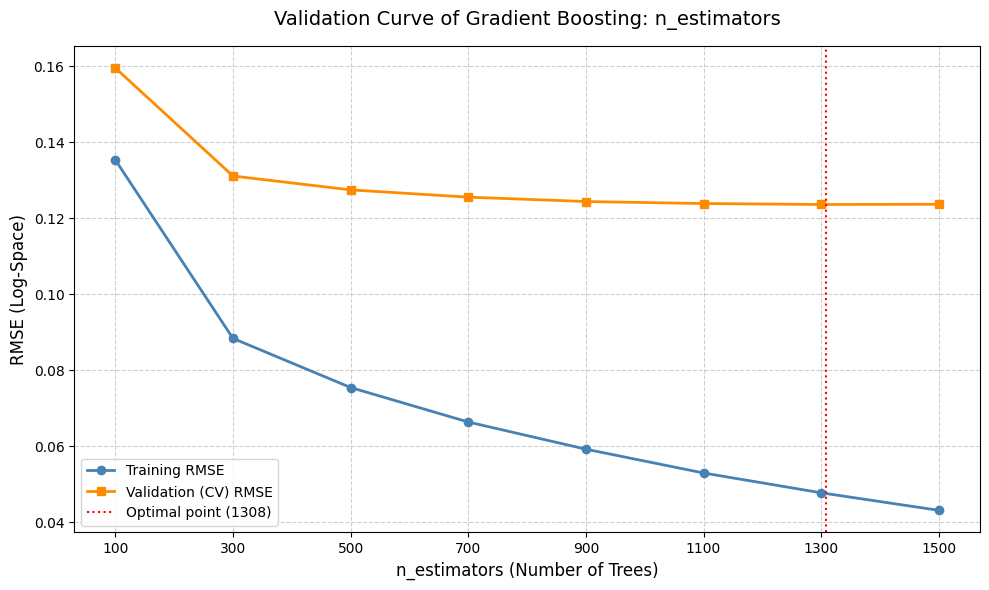
\includegraphics[width=\linewidth]{../picture/GB_n_estimater.png}
        \caption{Number of Estimators}
        \label{fig:vc_lr}
    \end{subfigure}\hfill
    \begin{subfigure}{0.45\textwidth}
        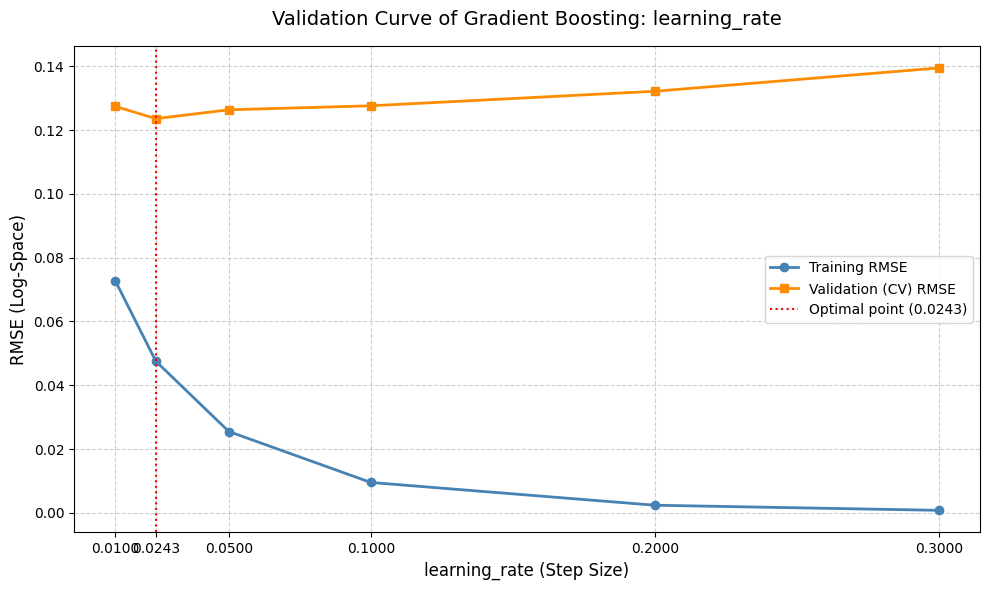
\includegraphics[width=\linewidth]{../picture/GB_learning_rate.png} % 注意檔名
        \caption{Learning Rate}
        \label{fig:vc_n_estimators}
    \end{subfigure}
    
    \vspace{0.3cm} % 增加排與排之間的垂直間距
    
    % 第二排
    \begin{subfigure}{0.45\textwidth}
        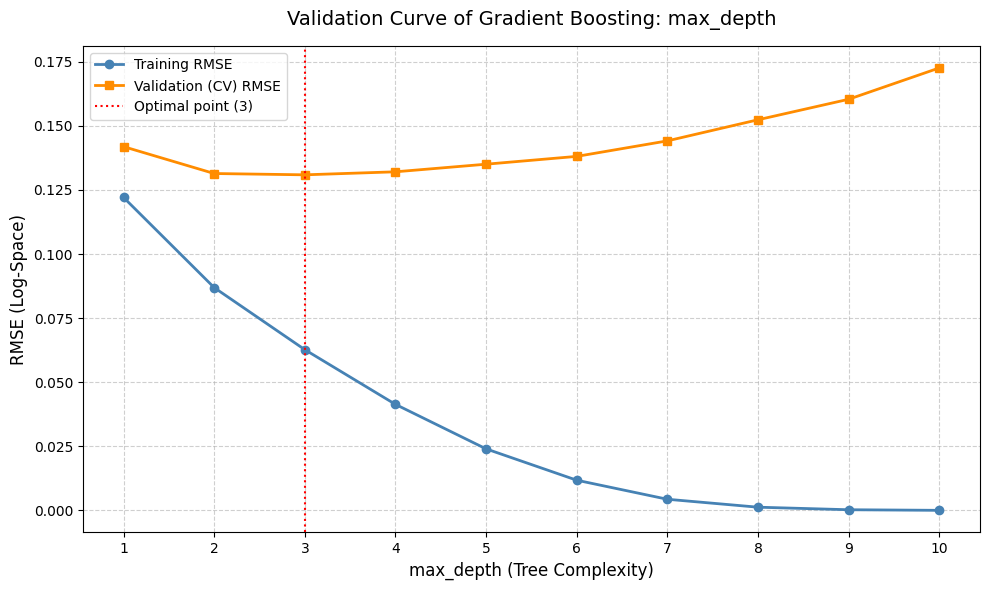
\includegraphics[width=\linewidth]{../picture/GB_max_depth.png}
        \caption{Maximum Depth}
        \label{fig:vc_max_depth}
    \end{subfigure}\hfill
    \begin{subfigure}{0.45\textwidth}
        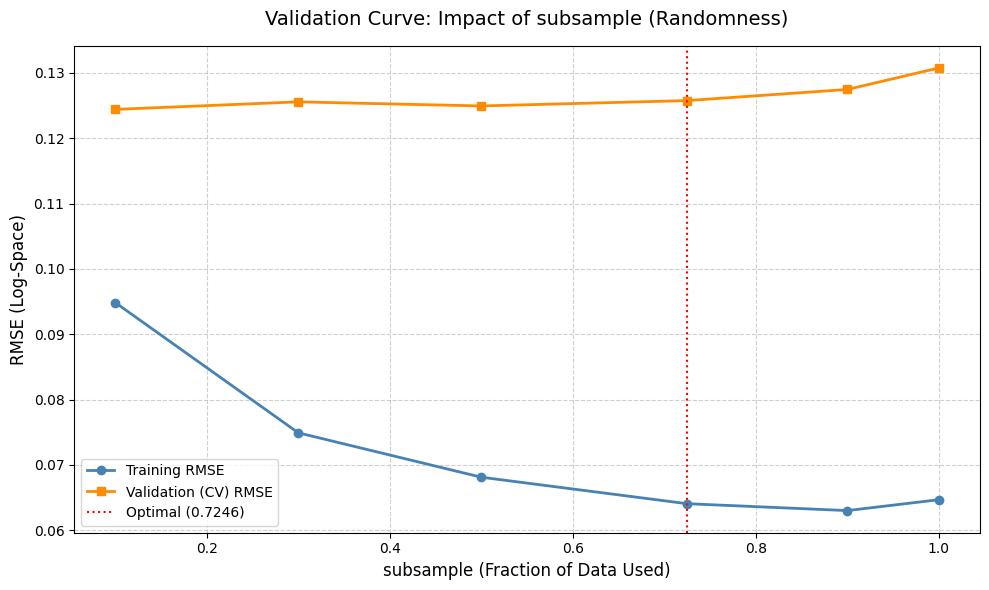
\includegraphics[width=\linewidth]{../picture/GB_sub_sample.png}
        \caption{Subsample Ratio}
        \label{fig:vc_subsample}
    \end{subfigure}
    
    \vspace{0.3cm}
    
    % 第三排
    \begin{subfigure}{0.45\textwidth}
        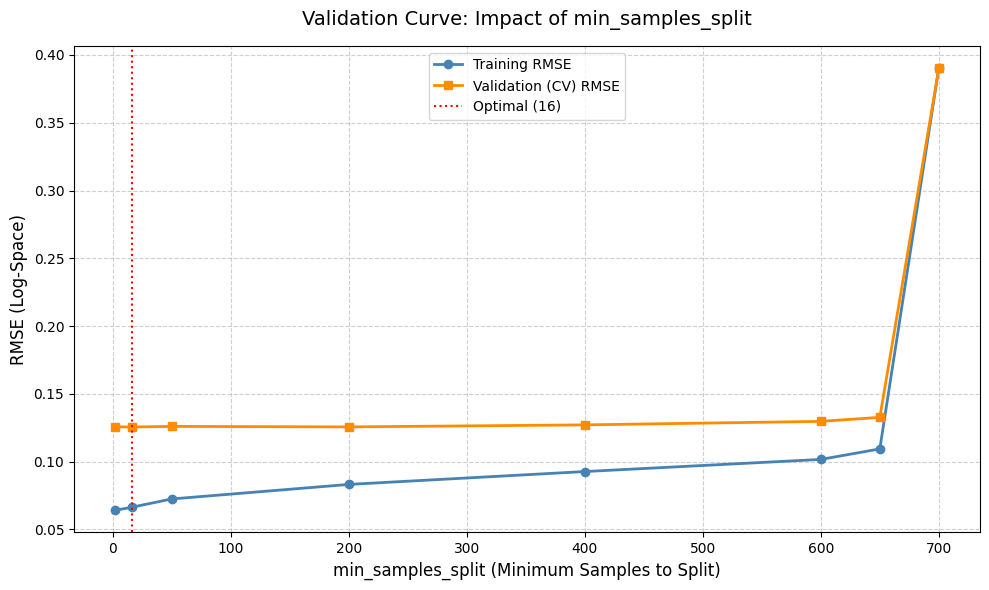
\includegraphics[width=\linewidth]{../picture/GB_min_sample_split.png}
        \caption{Min Samples Split}
        \label{fig:vc_min_split}
    \end{subfigure}\hfill
    \begin{subfigure}{0.45\textwidth}
        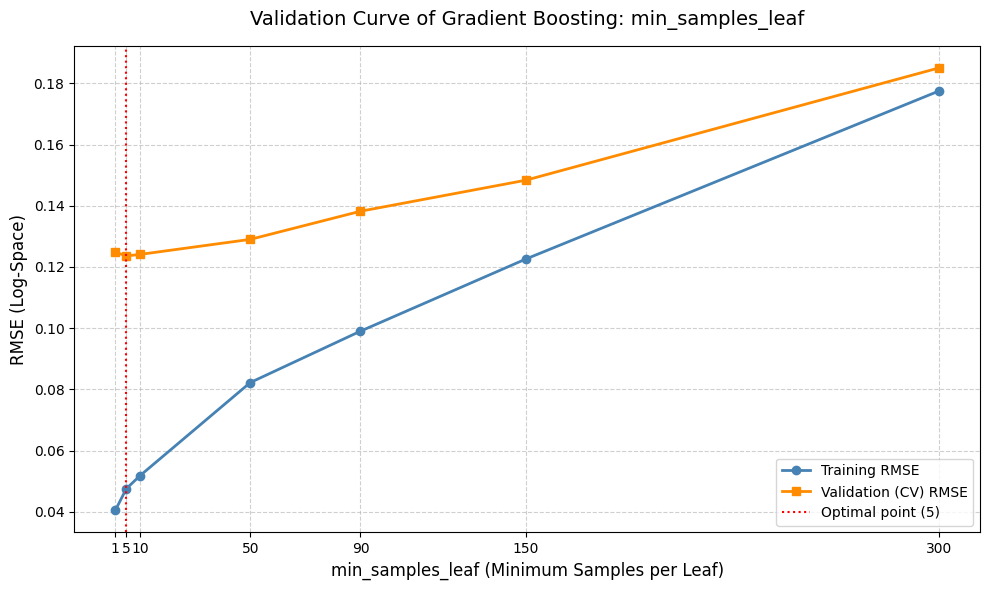
\includegraphics[width=\linewidth]{../picture/GB_min_sample_leaf.png}
        \caption{Min Samples Leaf}
        \label{fig:vc_min_leaf}
    \end{subfigure}

    \caption{Validation curves for the six key hyperparameters of the Gradient Boosting Regressor. The blue line represents the Training RMSE, while the orange line indicates the Validation (CV) RMSE. Vertical dotted lines mark the optimal parameters identified by the tuning process.}
    \label{fig:all_validation_curves}
\end{figure}

\subsubsection{Impact of Ensemble Size (n\_estimators)}

As shown in Figure \ref{fig:all_validation_curves}(a), the cross-validation error minimizes at \texttt{n\_estimators = 1308}. Because Gradient Boosting builds trees sequentially to correct prior errors, our small step size (\texttt{learning\_rate = 0.0243}) naturally requires a larger ensemble to achieve convergence.

However, the validation curve reveals a distinct plateau after approximately 700 trees, indicating \textbf{diminishing marginal returns}. By this point, the model has captured the primary predictive signals; subsequent learners contribute minimally, often fitting fine-grained residuals that represent irreducible noise.

While industrial applications involving large-scale data processing might truncate the ensemble at 700 trees to optimize efficiency, our dataset's small scale renders the computational overhead of 1308 trees negligible. Therefore, we retain the full 1308 estimators to strictly maximize predictive precision without compromising system performance.

\subsubsection{Impact of Step Size (learning\_rate)}

The validation curve for the learning rate, illustrated in Figure \ref{fig:all_validation_curves}(b), exhibits a classic U-shaped bias-variance tradeoff. We observe that the model achieves its minimum validation error at an optimal step size of \texttt{learning\_rate = 0.0243}.

When the learning rate is set below this learning rate, both training and validation errors remain relatively high. This indicates a state of \textbf{underfitting}. Conversely, as the learning rate increases beyond the optimal point, the training error continues to approach zero while the validation error steadily rises. This divergence clearly demonstrates \textbf{overfitting}; an excessively large step size causes the algorithm to aggressively memorize local noise in the training data, thereby degrading its generalization capability on unseen data.

\subsubsection{Impact of Tree Complexity (max\_depth)}

The validation curve for the maximum tree depth, shown in Figure \ref{fig:all_validation_curves}(c), explicitly demonstrates the relationship between model capacity and the bias-variance tradeoff. 

At lower depths (e.g., \texttt{max\_depth = 1}), the ensemble suffers from \textbf{underfitting}. The base learners are too shallow to capture the underlying non-linear relationships within the housing data, resulting in elevated error rates across both the training and validation sets. 

The validation error stabilizes in the region between depths 2 and 4, identifying \texttt{max\_depth = 3} as the optimal structural complexity. Conversely, as the tree depth increases beyond 4, the training error rapidly approaches zero while the validation error steadily ascends. This pronounced divergence indicates \textbf{overfitting}. Trees that are permitted to grow too deep construct overly complex decision boundaries, ultimately memorizing idiosyncratic noise and outliers in the training data rather than generalizing broader market trends.

\subsubsection{Impact of Subsample Ratio (subsample)}

This analysis evaluates the effect of \texttt{subsample} (the fraction of training instances randomly sampled to fit each individual base learner). As depicted in Figure \ref{fig:all_validation_curves}(d), the model's performance traverses three distinct phases, empirically validating the mathematical necessity of Stochastic Gradient Boosting:

\vspace{0.3cm} % 增加一點與前文的間距

\begin{enumerate}[label=\textbf{\arabic*.}, leftmargin=*, itemsep=0.4cm]
\item  \textbf{Information Deficit Zone (0.1 -- 0.3): Severe Underfitting} \\
At excessively low subsampling ratios (e.g., 10\%), the information available to each decision tree is highly fragmented. As observed, the training error reaches its global maximum in this zone, indicating a state of pronounced \textbf{high bias} and \textbf{underfitting} due to severe data restriction. Although this extreme stochasticity forcibly suppresses the validation error---creating a deceptively flat curve---this is merely a ``false convergence'' constrained by inadequate model capacity. In reality, the ensemble fails to adequately learn the deep, non-linear market features within the data, rendering configurations in this zone practically unusable.
\item  \textbf{Performance Sweet Spot and Algorithmic Convergence (0.5 -- 0.9)} \\
The validation error reaches its minimum plateau within the 0.5 to 0.9 range. Visually, the validation error at 0.5 appears marginally lower than at 0.7246 (a difference falling within a negligible statistical margin of $\sim 0.001$). However, the \texttt{RandomizedSearchCV} algorithm converged on \texttt{subsample = 0.7246} as the empirical optimum. We validated and retained this algorithmically derived value based on two rigorous scientific considerations:
\begin{itemize}
    \item \textbf{Global vs. Local Optimum:} The value 0.7246 represents a global optimum identified by \texttt{RandomizedSearchCV} operating across a high-dimensional hyperparameter space (accounting for interactions with learning rate, depth, etc.). Evaluating a single parameter slice merely reveals a local minimum, which ignores these crucial synergistic effects.
    \item \textbf{Information-Stochasticity Balance:} Retaining approximately 72\% of the data preserves a robust amount of structural housing information while injecting sufficient randomness. This balance provides more stable predictions than aggressively discarding half of the dataset (i.e., 0.5).
\end{itemize}
\item  \textbf{Loss of Stochastic Protection (1.0): Ensemble Overfitting} \\
At \texttt{subsample = 1.0}, stochastic sampling is disabled, forcing all trees to train on the exact same data. The resulting divergence---where training error continues downward while validation error rebounds---demonstrates that these highly correlated trees collectively memorize the same noise. Introducing stochasticity (e.g., 0.7246) effectively breaks this correlation, acting as a crucial regularization mechanism against ensemble overfitting.
\end{enumerate}

\subsubsection{Impact of Split Threshold: Asymmetric Growth (\texttt{min\_samples\_split})}

The validation curve for \texttt{min\_samples\_split} (Figure \ref{fig:all_validation_curves}(e)) shows remarkable stability up to a threshold of 600, before experiencing a catastrophic underfitting cliff at 700. This phenomenon yields two profound insights into the model's architecture:

\begin{itemize}[itemsep=0.2cm, topsep=0.2cm, leftmargin=*]
    \item \textbf{Asymmetric Splitting under Draconian Constraints:} Driven by impurity reduction, decision trees frequently isolate small subsets of outliers while retaining most instances in a dominant ``trunk'' node. A high threshold (e.g., 600) halts minority nodes but allows the trunk node to grow deeper, explaining the model's resilience.
    \item \textbf{Reverse-Engineering Topology:} The sudden collapse at 700 reveals that the maximum sample mass of the primary root nodes lies between 650 and 700. Surpassing this critical mass paralyzes the tree-building process at the root, reducing the ensemble to non-functional stumps.
\end{itemize}

\subsubsection{Impact of Leaf Size: Theoretical Limits (\texttt{min\_samples\_leaf})}

At \texttt{max\_depth = 3}, a perfectly symmetric tree contains up to $2^3 = 8$ leaves. Distributing our 1,168 training samples yields a theoretical average capacity of exactly 146 samples per leaf. The validation curve (Figure \ref{fig:all_validation_curves}(f)) empirically corroborates this mathematical boundary through extreme stress testing. Setting \texttt{min\_samples\_leaf = 150} marginally exceeds this natural limit, triggering premature early stopping and an observable upward inflection in error. Furthermore, an aggressive threshold of 300 mathematically restricts the base learners to a maximum of three leaves ($1168 \div 300 \approx 3.89$), completely obliterating the depth-3 architectural advantage and causing severe underfitting. This destructive testing justifies our final permissive configuration (\texttt{leaf = 5}), which provides essential regularization against noise while fully unleashing the model's structural capacity.

\section{Model Evaluation and Feature Importance}

Having completed the comprehensive hyperparameter optimization, we can now conduct an in-depth comparison of the optimized Gradient Boosting Regression (GBR) model against the regularized linear baselines (Lasso and Ridge). By juxtaposing their internal stability and external generalization capabilities, we clearly establish the algorithmic superiority of the ensemble approach before delving into the interpretability and feature importance of the model.

\subsection{Comparative Performance: Stability and Generalization}

% --- 兩張圖並排顯示區塊 (放在 subsection 正下方) ---
\begin{figure}[H]
     \centering
     \begin{subfigure}[b]{0.48\textwidth}
         \centering
         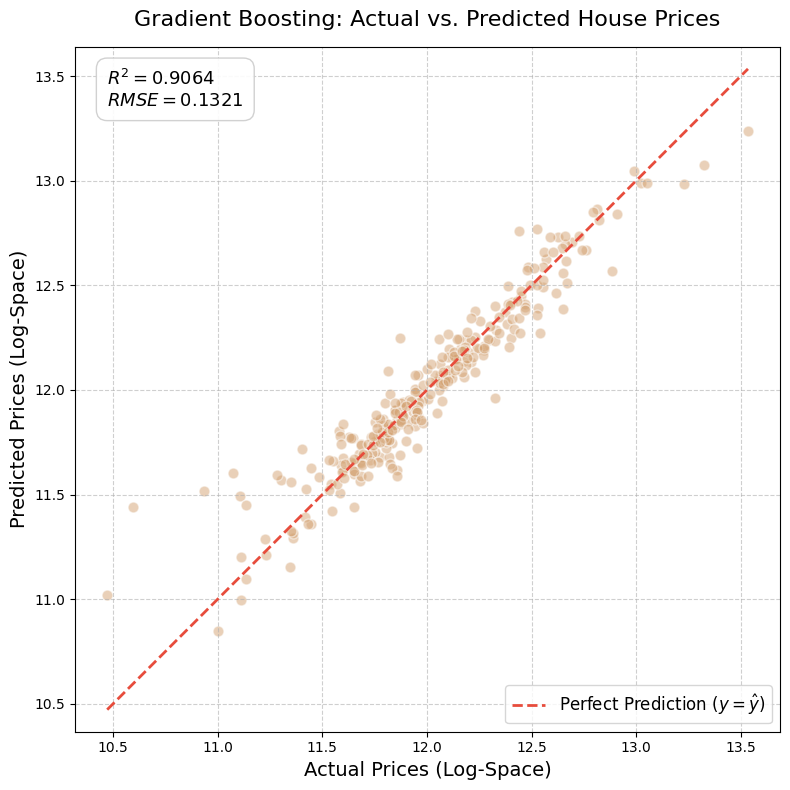
\includegraphics[width=\textwidth]{../picture/GB_predict_actual.png}
         \caption{GBR Actual vs. Predicted Plot}
         \label{fig:GB_pred_actual}
     \end{subfigure}
     \hfill
     \begin{subfigure}[b]{0.48\textwidth}
         \centering
         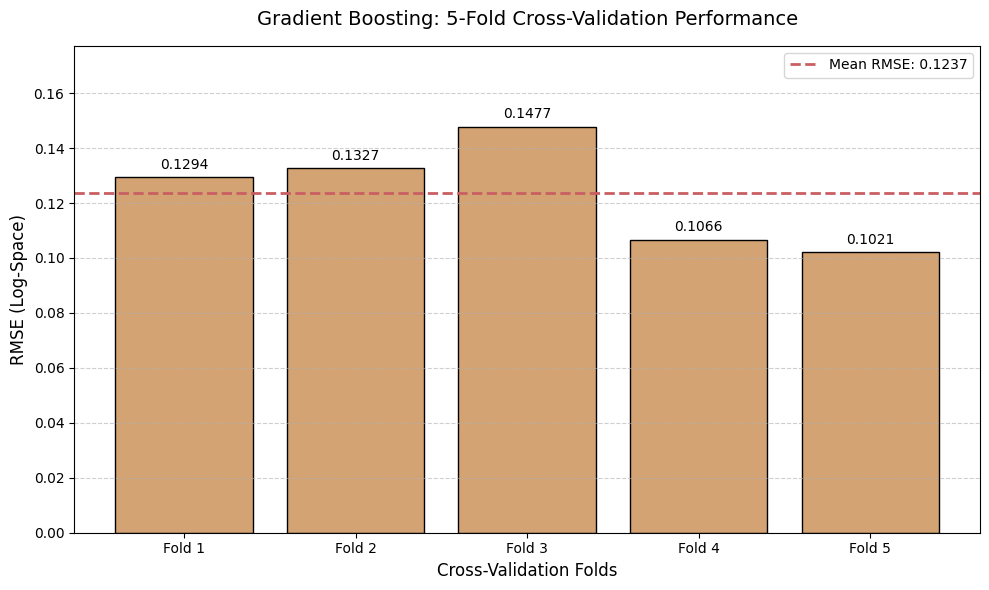
\includegraphics[width=\textwidth]{../picture/GB_cross_validation.png}
         \caption{GBR 5-Fold Cross-Validation Scores}
         \label{fig:GB_cv_scores}
     \end{subfigure}
     \caption{Diagnostic visualizations of the GB model, illustrating high variance and weight instability.}
     \label{fig:GB_diagnostics}
\end{figure}

% ----------------------------------------------------

\textbf{1. Internal Stability via Cross-Validation} \\
Figure \ref{fig:GB_cv_scores} illustrates the 5-fold cross-validation performance of our optimized GBR model. The ensemble achieved a highly competitive mean RMSE of 0.1237. More importantly, when compared to the linear baselines (e.g., Ridge, which exhibited a severe error spike of 0.2037 in Fold 3), the GBR model demonstrates remarkable fold-to-fold stability. The narrow variance across different data splits confirms that the sequential error-correction mechanism of boosting effectively mitigates the risk of overfitting to idiosyncratic subsets of the training data, yielding a highly robust architecture.

\vspace{0.3cm}

\textbf{2. External Generalization on Unseen Data} \\
The ultimate test of a predictive model lies in its generalization capability on unseen testing data. Figure \ref{fig:GB_pred_actual} presents the Actual vs. Predicted scatter plot for the GBR model. The predictions cluster tightly along the red identity line ($y = \hat{y}$), culminating in an impressive $R^2$ score of 0.9064 and a test RMSE of 0.1321. 

In contrast to Ridge regression ($R^2 = 0.8974$, RMSE = 0.1384), the Gradient Boosting ensemble exhibits noticeably less dispersion, particularly in the mid-to-high price ranges. This performance gap highlights a fundamental theoretical advantage: while Lasso and Ridge are constrained by linear assumptions, the tree-based GBR model successfully captures deep, non-linear feature interactions (e.g., the synergistic effect of neighborhood quality and living area) without requiring manual polynomial feature engineering. 

Although noticeable deviations remain at the lower tail of the price distribution (i.e., lower-tier properties) likely due to unobserved idiosyncratic factors such as severe disrepair or distressed sales, the overall predictive precision confirms GBR as the superior model. With the predictive accuracy established, the following sections will open this algorithmic ``black box'' to analyze feature importance and masking effects.

\subsection{Feature Importance and Model Interpretability: Opening the Black Box}

To elucidate the decision-making process of our models, we extract and compare the feature importances from the optimized Gradient Boosting model (based on impurity reduction) alongside the coefficient weights from the regularized linear models (Lasso and Ridge). 

% ==========================================
% 第一部分：放在前一頁的圖 (a)
% ==========================================
\begin{figure}[htbp] % 這裡可以用 htbp 讓它自然浮動，或用 H 強制固定
    \centering
    \begin{subfigure}[b]{0.75\textwidth}
        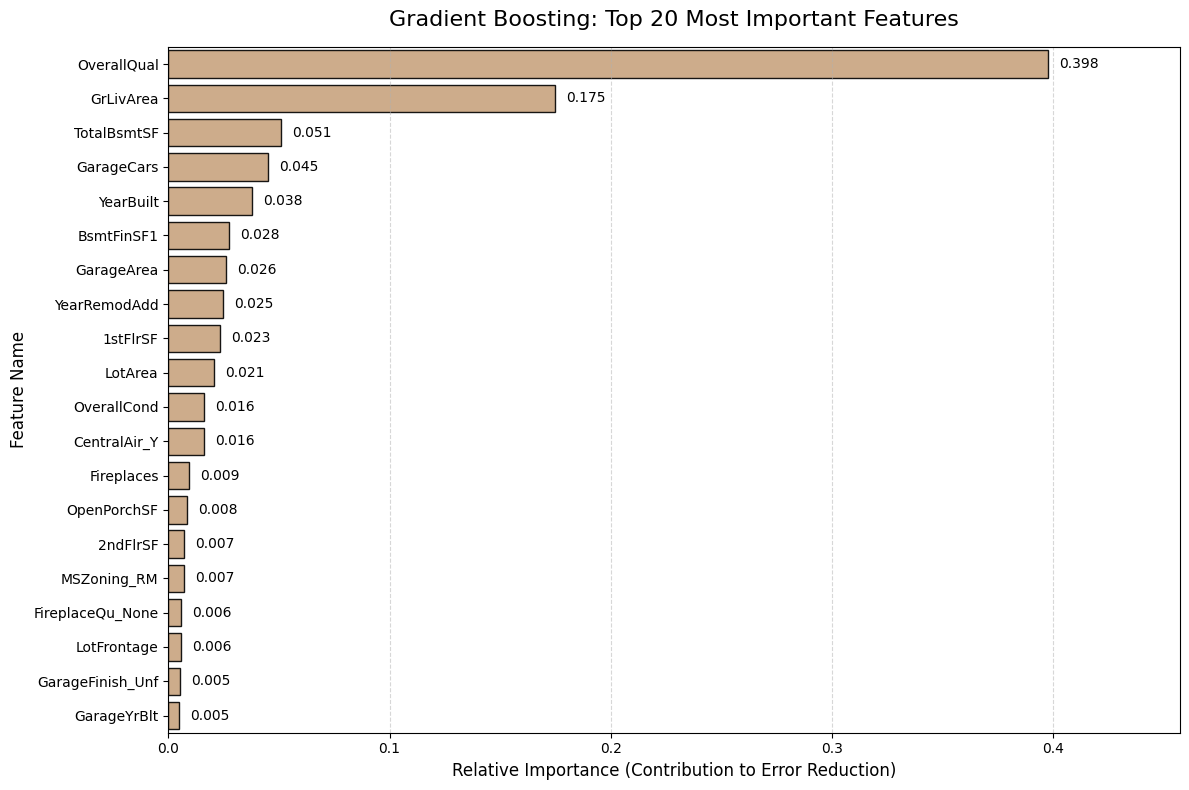
\includegraphics[width=\linewidth]{../picture/GBR_influential_features_yellow.png} 
        \caption{Gradient Boosting}
    \end{subfigure}
    \caption{Cross-Algorithm Comparison of Feature Influences (Part 1).}
    \label{fig:linear_nonlinear_feature_comparison_1}
\end{figure}

% 💡 這裡可以穿插你在 5.5 節的說明文字...
% 這樣文字就會自然地填補在圖 (a) 的下方，不會浪費版面。

% ==========================================
% 第二部分：放在下一頁的圖 (b) 與 (c)
% ==========================================
\begin{figure}[H]
    \ContinuedFloat % 🌟 魔法指令：讓編號接續上一張圖！
    \centering
    
    \begin{subfigure}[b]{0.75\textwidth}
        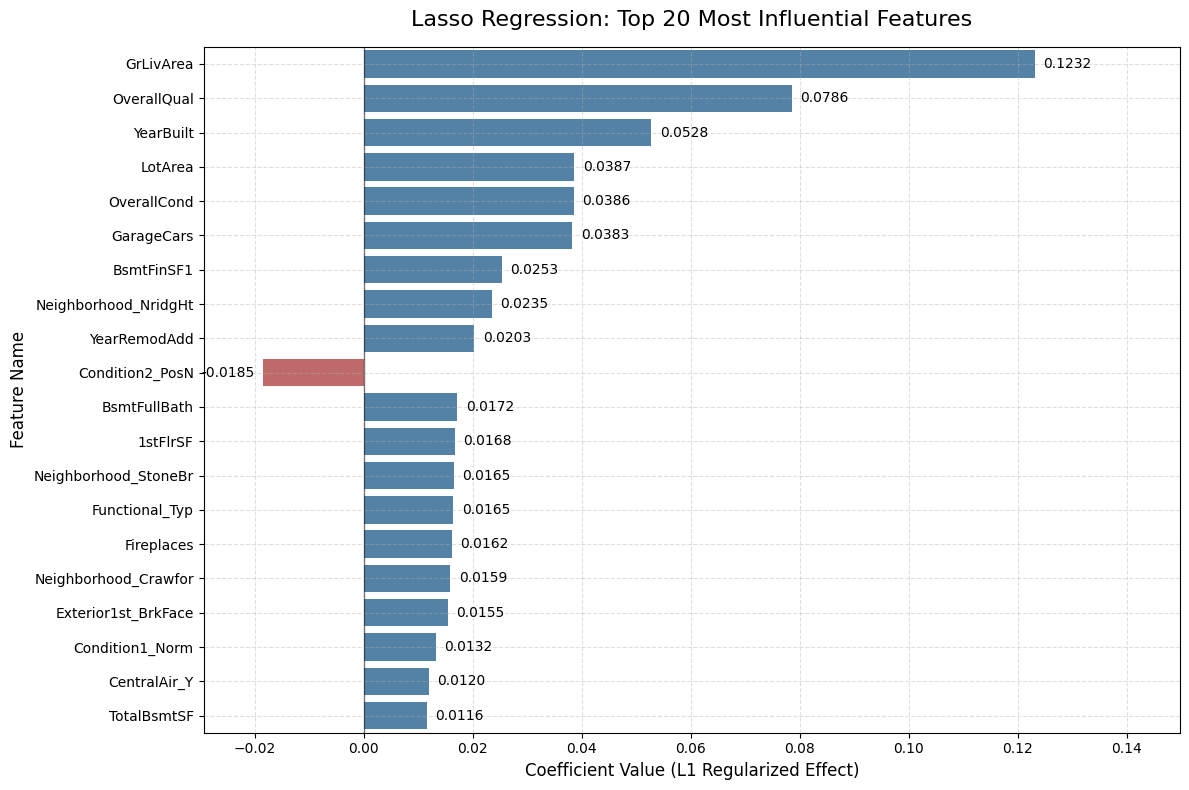
\includegraphics[width=\linewidth]{../picture/lasso_influential_features.png} 
        \caption{Lasso Regression}
    \end{subfigure}
    
    \vspace{0.3cm} % 稍微增加一點間距讓畫面不擁擠
    
    \begin{subfigure}[b]{0.75\textwidth}
        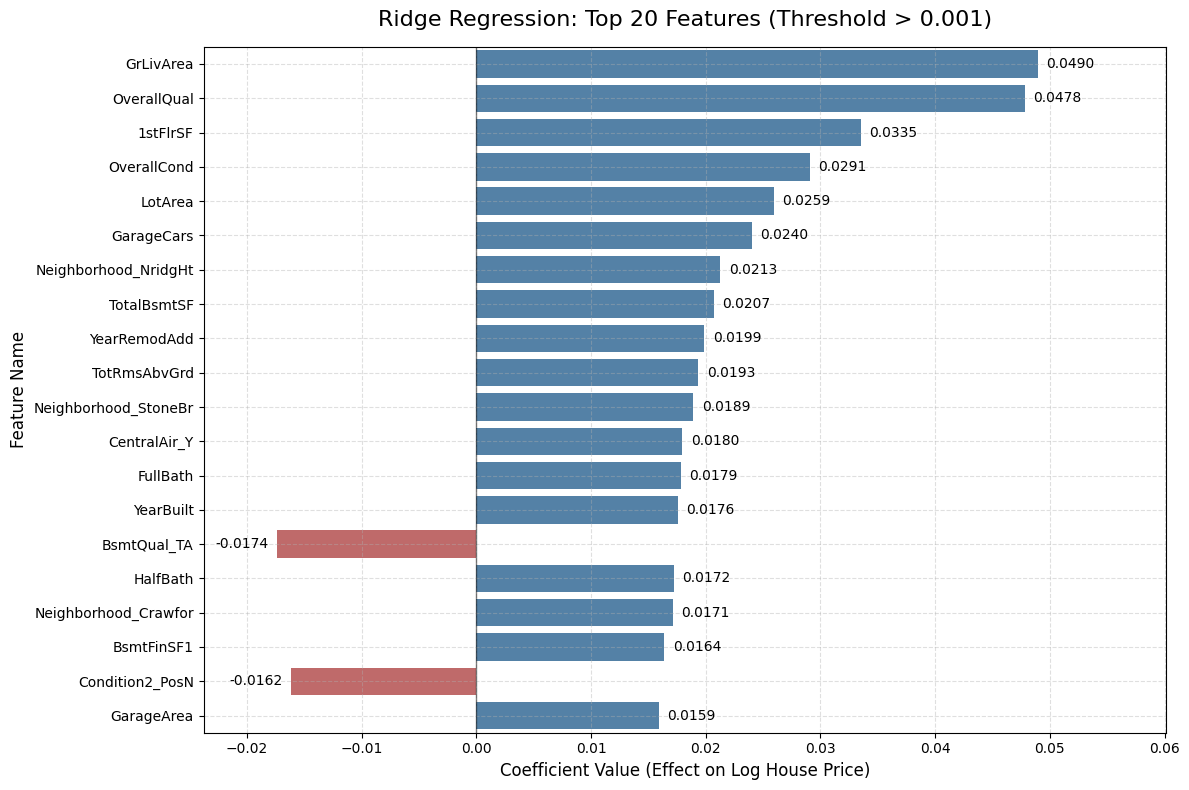
\includegraphics[width=\linewidth]{../picture/Ridge_influential_features.png} 
        \caption{Ridge Regression}
    \end{subfigure}
    
    \caption{Cross-Algorithm Comparison of Feature Influences (Continued). Subfigures (b) and (c) display the coefficient distribution for the regularized linear models.}
    \label{fig:linear_nonlinear_feature_comparison_2}
\end{figure}

As illustrated in Figure \ref{fig:linear_nonlinear_feature_comparison_1}, the cross-algorithm comparison reveals a striking consensus on the core drivers of property value, alongside fundamental mechanical differences in how each algorithm allocates predictive power. We distill these algorithmic behavioral differences into three core observations:

\vspace{0.3cm}
\begin{enumerate}[label=\textbf{\arabic*.}, leftmargin=*]
\item \textbf{Algorithmic Consensus on Core Value Drivers} \\
Unlike unregularized linear models that often hyper-fixate on sparse categorical variables, our optimized models exhibit perfect alignment on the most critical structural metrics. Across all three architectures, the overall finish quality (\texttt{OverallQual}) and the above-ground living area (\texttt{GrLivArea}) decisively dominate the top positions. This consensus validates our preprocessing pipeline and confirms that regardless of the underlying mathematical assumptions (linear vs. non-linear), these two fundamental metrics dictate the baseline valuation in the Ames housing market.

\vspace{0.3cm}

\item \textbf{Concentration vs. Distribution of Predictive Power} \\
While the models agree on \textit{what} is important, they differ drastically in \textit{how} they distribute importance. Figure \ref{fig:feat_gbr} demonstrates that GBR's greedy splitting mechanism creates an extreme concentration of predictive power—\texttt{OverallQual} alone accounts for nearly 40\% of the impurity reduction. In stark contrast, the regularized linear models (Figures \ref{fig:feat_lasso} and \ref{fig:feat_ridge}) explicitly penalize extreme coefficients. Ridge, in particular, enforces a highly symmetric distribution, capping its maximum coefficient at 0.0490 and distributing the predictive burden smoothly across a broader range of variables (e.g., \texttt{1stFlrSF}, \texttt{LotArea}).

\vspace{0.3cm}

\item \textbf{Mechanisms of Collinearity: The Garage Paradigm} \\
The comparison provides a textbook demonstration of how different algorithms resolve multicollinearity, perfectly illustrated by the highly correlated \texttt{GarageCars} (capacity) and \texttt{GarageArea} (square footage) features. In the tree-based GBR model (a), both features provide distinct information gain at different tree depths, though \texttt{GarageCars} (0.045) takes precedence. The linear models, however, diverge sharply based on their penalty terms. Lasso regression (b), driven by its L1 penalty, aggressively enforces sparsity—it selects \texttt{GarageCars} (0.0383) as the dominant predictor and completely eliminates \texttt{GarageArea} from the top 20 influential features. Ridge regression (c), governed by its L2 penalty, symmetrically shrinks and retains both (\texttt{GarageCars} at 0.0240 and \texttt{GarageArea} at 0.0159) to maintain mathematical stability.

\vspace{0.3cm}

\item \textbf{Resolution of the Sparse Outlier Anomaly} \\
Finally, this visual comparison perfectly validates our primary motivation for transitioning to a tree-based ensemble (as outlined in Section 5.1). In the linear models (b and c), the sparse categorical variable \texttt{Condition2\_PosN} retains a prominent, counter-intuitive negative penalty (represented by the red bars) to accommodate the extreme outlier, ID 524. Strikingly, \texttt{Condition2\_PosN} is entirely absent from the top 20 features of the GBR model (a). Because Gradient Boosting relies on hierarchical space partitioning, it naturally isolates ID 524 into a specific terminal leaf based on its unique combinations of area and neighborhood, without globally penalizing the park proximity feature. This absence confirms that GBR successfully eradicated the pathological weight distortions caused by idiosyncratic market anomalies.
\end{enumerate}

\section{Conclusion}
% 總結最終 RMSE 指標與商業價值

\end{document}